\documentclass{article}
\usepackage{tikz}

\begin{document}
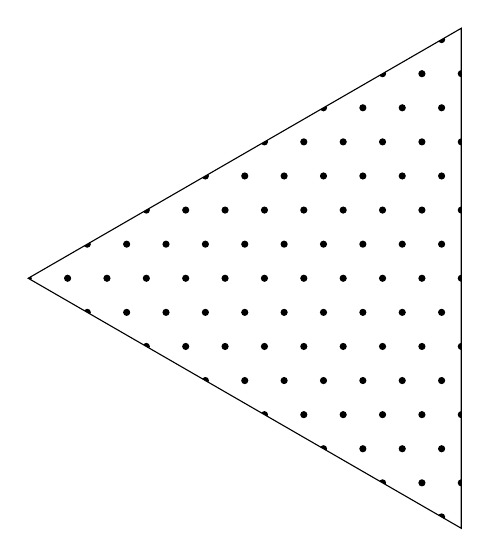
\begin{tikzpicture}[scale=.5]
\clip[draw] (-7,0)--(4, 3.66666*1.7320508)--(4, -3.66666*1.7320508)--cycle; 
\foreach \x in {-14,-13,...,14}{% Two indices running over each
    \foreach \y in {-10,-9,...,10}{% node on the grid we have drawn
        \draw[black, fill=black] (\x-\y/2,1.7320508*\y/2) circle (.5ex);}}

\end{tikzpicture}






\end{document}
